\newpage
\subsection{Creazione di un Biglietto}

Per la creazione di un Biglietto, necessario per permettere ai Viaggiatori di poter raggiungere una destinazione, ho utilizzato un algoritmo che coinvolge le componenti (distribuite) introdotte in sezione \ref{subsec:ticket_offices}.

Di seguito viene riportata una descrizione delle fasi previste dalla soluzione progettata.

	\subsubsection {Richiesta di Creazione}\label{subsubsec:ticket_creation_request}
	
	La richiesta di creazione di un \ttt{Ticket} da parte di un Viaggiatore, viene operata da un thread appartenente al pool di \ttt{Traveler\_Pool} che esegue l'operazione \ttt{CREATE\_TICKET} (come descritto precedentemente in sezione \ref{subsubsec:buy_ticket}). Tale operazione, effettua una richiesta di creazione alla biglietteria interna alla stazione di partenza $S$, la quale richiederà la creazione effettiva alla Biglietteria Regionale, se lo stesso \ttt{Ticket} non è presente in una cache locale.  
	
	\subsubsection {Creazione del Ticket} \label{subsubsec:ticket_creation}
	
	\begin{figure}[htbp]
		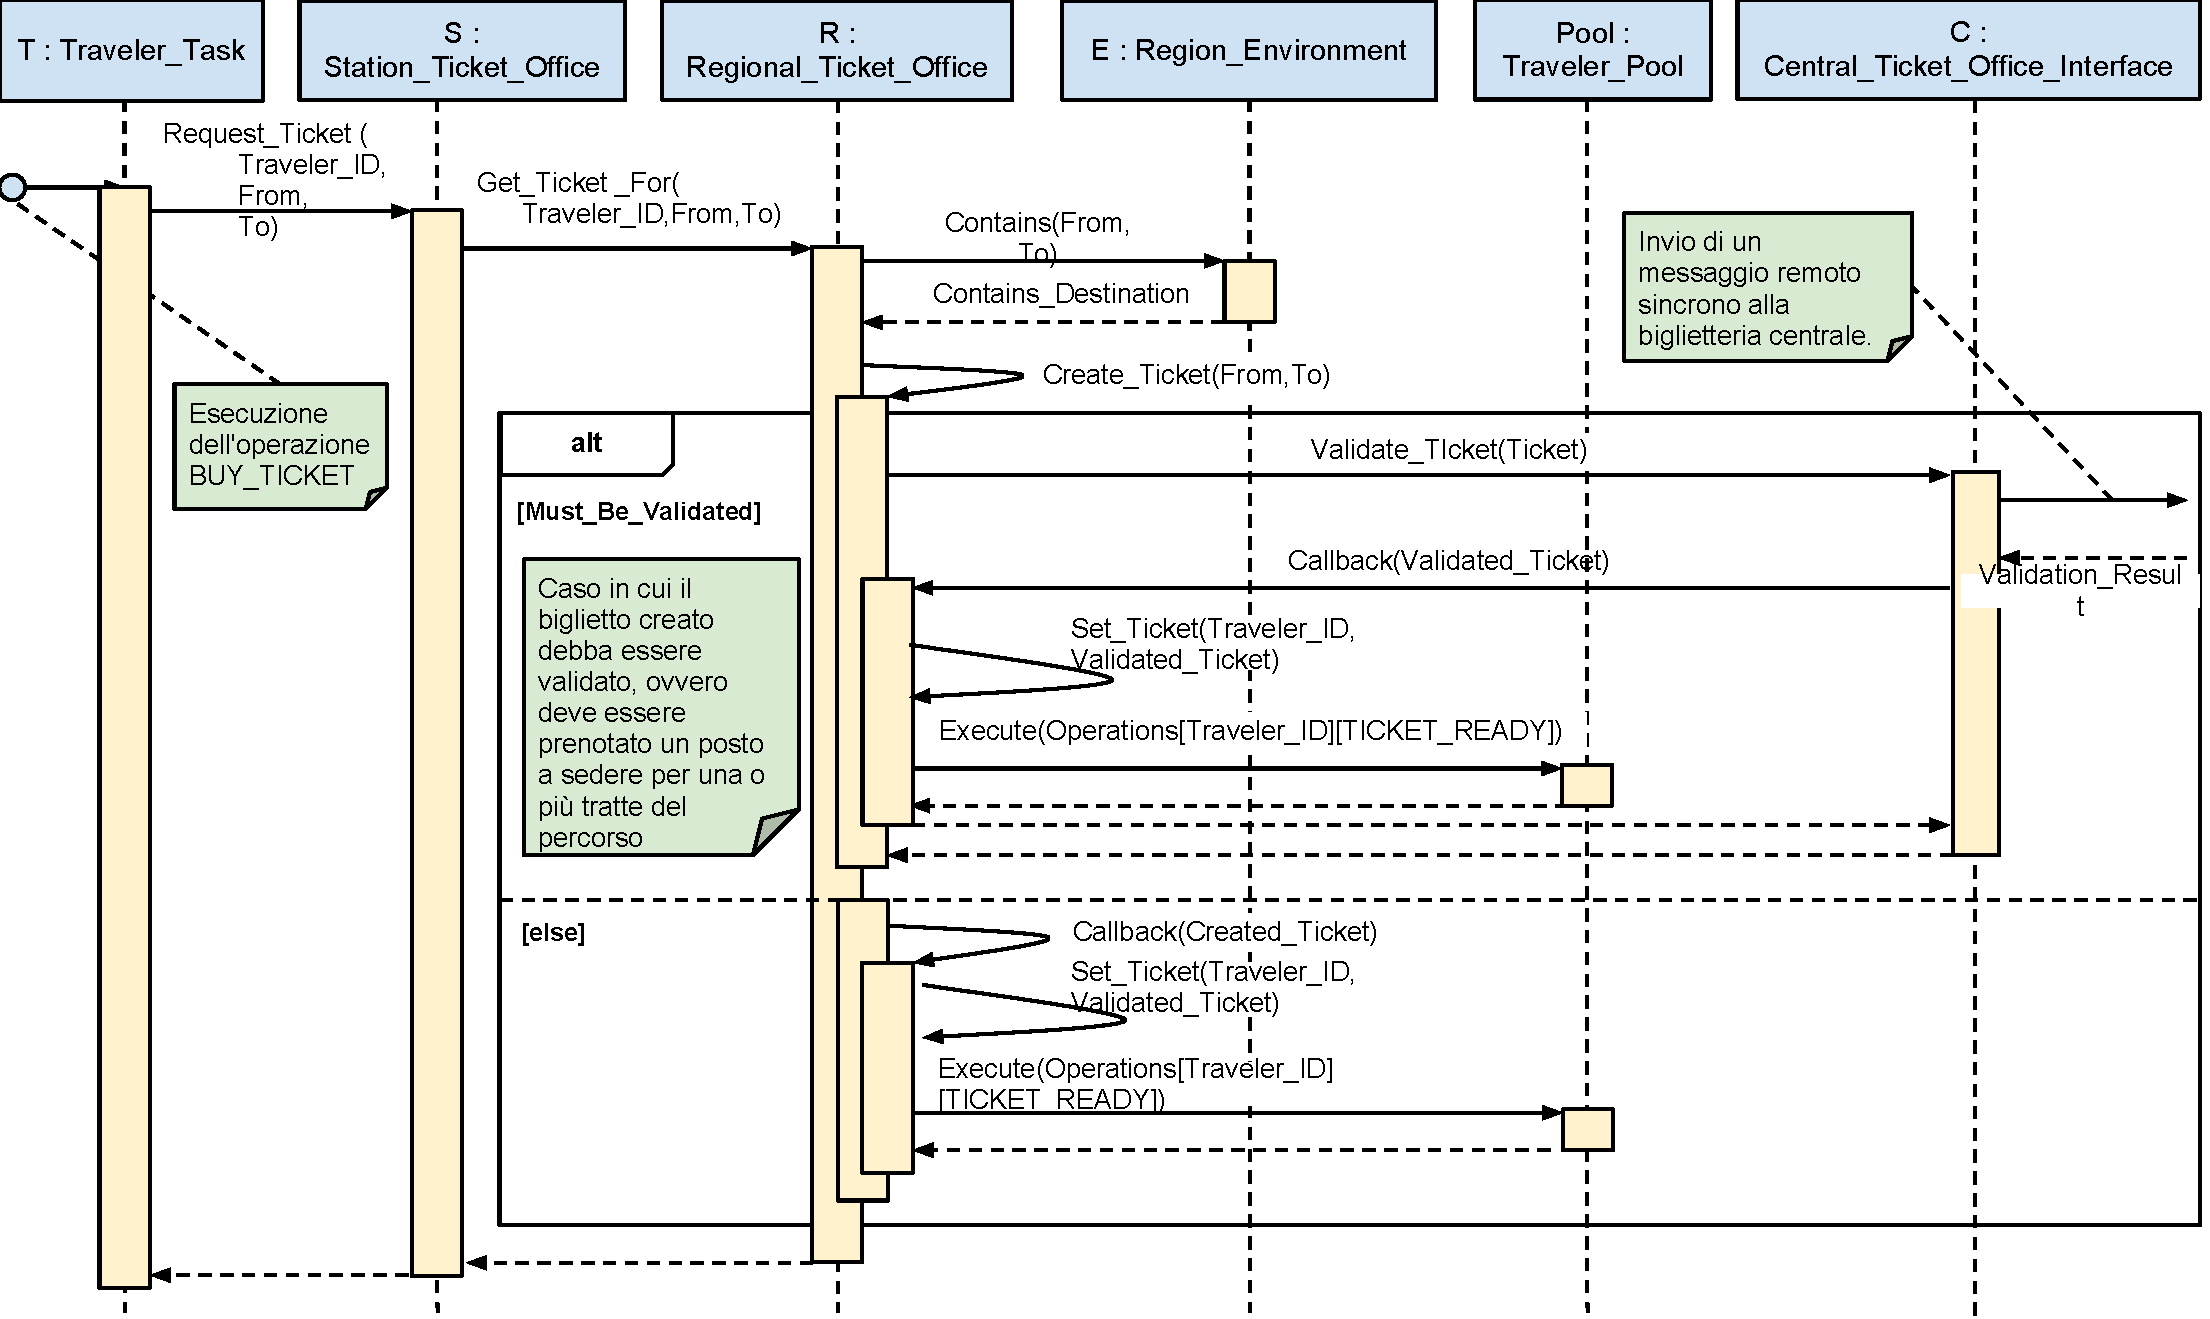
\includegraphics[trim = 55mm 0mm 0mm 0mm,scale=0.5]{imgs/Buy_Ticket_Sequence_Diagram.pdf}
		\caption{\footnotesize{Diagramma di Sequenza, creazione di un Ticket per una destinazione \ii{locale} alla regione di partenza.}}
		\label{fig:local_ticket_creation_diagram}
	\end{figure}
	
	Siano \ttt{From} e \ttt{To} rispettivamente l'identificativo della Stazione di partenza, e l'identificativo della Stazione di destinazione. Le operazioni svolte dalla Biglietteria Regionale sono:
	\begin{itemize}
		\item Se \ttt{To} appartiene alla Regione corrente, viene creato il \ttt{Ticket}, effettuando le seguenti operazioni:
			\begin {itemize}
					
				\item Si considera il percorso più breve da \ttt{From} a \ttt{To}, che indicheremo con $Path = \{s_1,...,s_N\}$. Questo percorso è ottenuto applicando un semplice algoritmo di cammino minimo sul grafo avente come vertici le Stazioni, e come archi non direzionati i Segmenti che li collegano. Il cammino può minimizzare, ad esempio, la lunghezza totale del percorso.
				
				\item Il percorso $Path$ viene intersecato con i Percorsi dei Treni (\ttt{Route}), per poter definire le Tappe che compongono il Biglietto. Sia $i=1$, allora finché $i<=N$:
					\begin{itemize}
						\item Ottieni i percorsi dei Treni (\ttt{Route}s) $R={r_1,...,r_k}$ che contengono una Tappa $t$ tale per cui i campi \ttt{Start\_Station} e \ttt{Next\_Station} sono rispettivamente $s_i$ e $s_{i+1}$. Per ciascuno di questi percorsi, vengono ottenuti indice e posizione della tappa $t$ al suo interno.
						A questo punto si procede all'individuazione del percorso che meglio si adatta al cammino minimo da seguire. Sia quindi $k = i$; per ciascuna route $r_j \in R$, a partire dalla posizione di $t$ in $r_j$, si procede ad estendere la corrispondenza. Viene quindi mantenuto il percorso con la corrispondenza di lunghezza massima $Max\_Length$, memorizzandone l'indice in $Max\_Match$.
						\item Una volta stabilita la corrispondenza di lunghezza massima, viene creata una Tappa del \ttt{Ticket}:
						\begin{verbatim}
							- start_station        : indice della stazione 
							                         di inizio dell'estensione;
							- next_station         : indice della stazione di
							                         fine dell'estensione 
							                         massima;
							- train_id             : indice del Treno che 
							                         percorre il percorso di 
							                         indice Max_Match;
							- start_platform       : indice della Piattaforma
							                         di partenza in t;
							- destination_platform : indice della Piattaforma 
							                         dell'ultima tappa;
							- run_number           : identificativo della Corsa 
							                         per la quale si effettua 
							                         prenotazione. Inizialmente 
							                         viene messa a 0 e modificata 
							                         successivamente se necessario; 
							- next_region          : regione corrente.
							
						\end{verbatim}
						\item $i$ viene incrementato di $Max\_Length$, per poter procedere all'individuazione della prossima corrispondenza di lunghezza massima.
					\end{itemize} 
			\item Una volta creato il \ttt{Ticket}, allora se esso conterrà almeno una Tratta che prevede l'utilizzo di un Treno a prenotazione (ovvero di tipo \ttt{FB}), allora si dovrà procedere alla \ii{Validazione}, descritta nella sezione \ref{subsubsec:validation}.
			\item Altrimenti, il \ttt{Ticket} creato viene assegnato al Viaggiatore e viene quindi inserita l'operazione \ttt{TICKET\_READY} nella coda di operazioni di \ttt{Traveler\_Pool}.
			\end {itemize} 
		\item Se \ttt{To} non appartiene alla Regione corrente, allora viene effettuata una richiesta remota alla Biglietteria Centrale. \'E opportuno che la richiesta di creazione sia asincrona, in modo tale da permettere al thread che la effettua di non dover attendere attivamente per una risposta, e quindi di poter eseguire altre operazioni eventualmente presenti nella coda di \ttt{Traveler\_Pool}.
	\end{itemize} 
	
	In figura \ref{fig:local_ticket_creation_diagram} è riportato un diagramma di sequenza che presenta le operazioni svolte per la creazione di un Ticket locale alla Regione dalla quale la richiesta è effettuata. 


	\subsubsection {Richiesta di Creazione Remota}\label{subsubsec:remote_ticket_creation}
	
	
	\begin{figure}[htbp]
		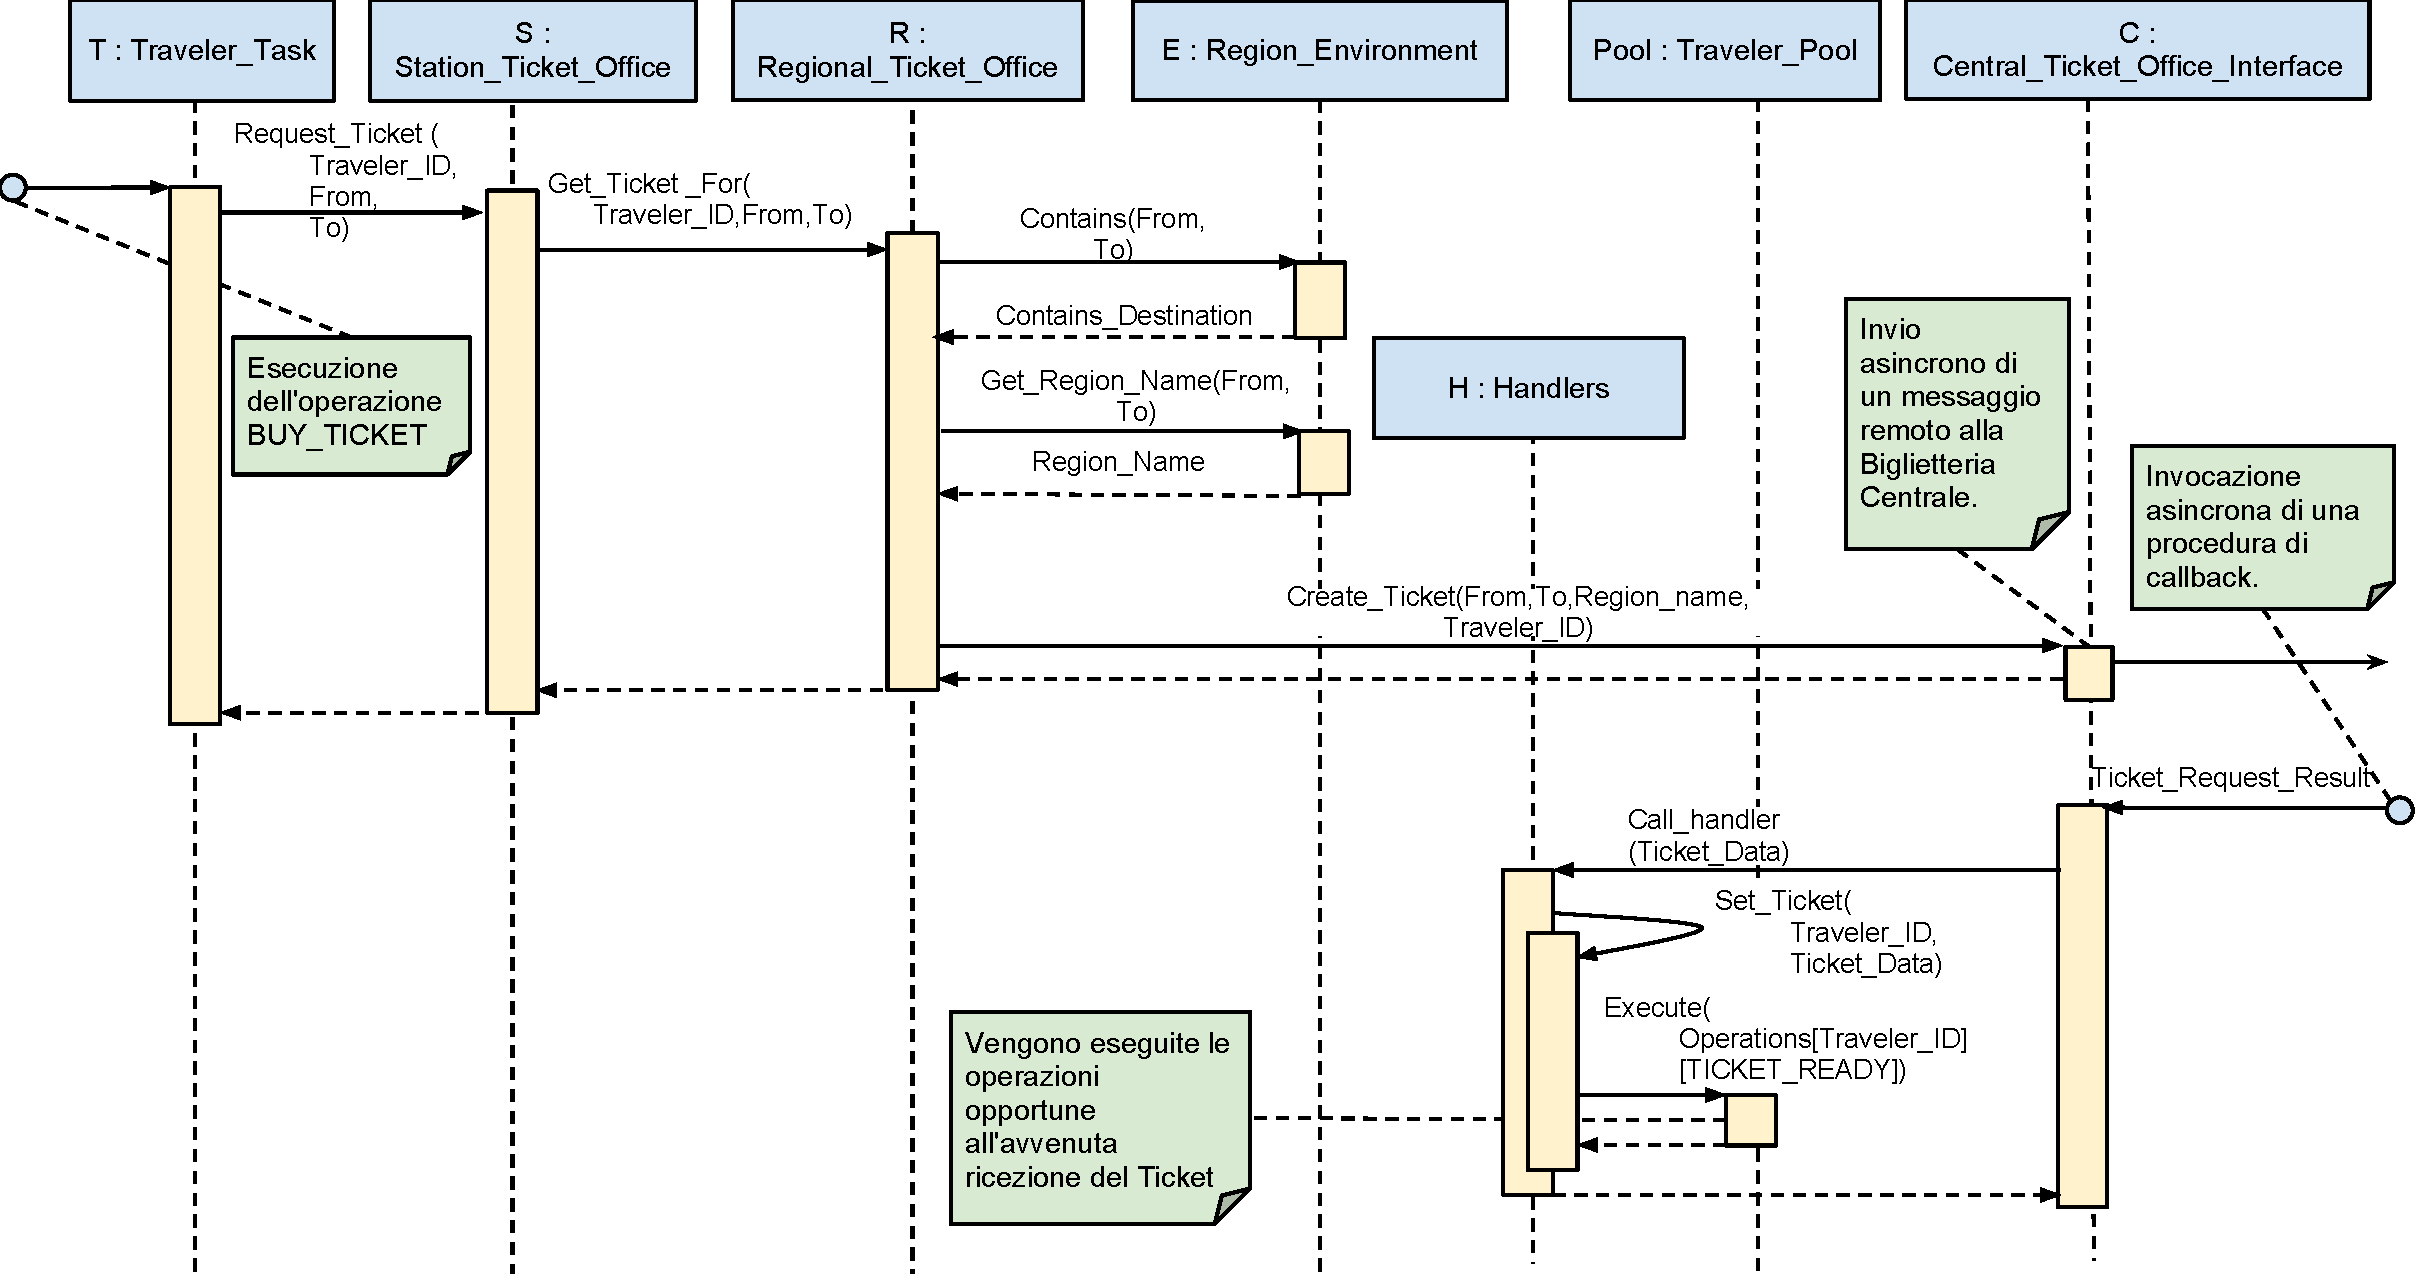
\includegraphics[trim = 55mm 0mm 0mm 0mm,scale=0.5]{imgs/Buy_Ticket_Sequence_Diagram_Remote.pdf}
		\caption{\footnotesize{Diagramma di Sequenza, creazione di un Ticket per una destinazione \ii{non appartenente} alla regione di partenza.}}
		\label{fig:remote_ticket_creation_diagram}
	\end{figure}
	
	
	Una volta che la Biglietteria Centrale riceve, tramite l'interfaccia remota esposta, un messaggio remoto di richiesta di Creazione di un Biglietto, essa effettua 3 operazioni:
	\begin{itemize}
		\item Individua la Regione di appartenenza della destinazione $To$; se tale informazione non è presente nella cache locale mantenuta dalla Biglietteria Centrale, essa viene ricercata nel modo seguente: 
			\begin{itemize}
				\item viene recuperato l'elenco completo delle Regioni (ovvero una lista di coppie \ttt{(Node\_Name,Node\_Address)}) dal \ii{Server dei Nomi};
				\item per ciascun elemento dell'elenco, viene inviato un messaggio remoto, al quale ciascuna Regione risponde con \ttt{True}, se contiene la Stazione, o \ttt{False} in caso contrario.
			\end{itemize}
		\item Se nessuna risposta positiva viene ricevuta, allora viene comunicato l'errore alla Biglietteria Regionale richiedente, inviando un messaggio di errore.
		\item Nel caso in cui si abbia una risposta positiva da una Regione $R$ allora:
			\begin{itemize}
				\item Viene recuperata la lista $R_1,...,R_n$ di Regioni attraverso le quali costruire il percorso per raggiungere la destinazione (dalla mappa \ttt{Links}). 
				\item Per ciascuna Regione $R_i$ viene inviata una richiesta remota \ii{sincrona} per ottenere un Ticket che collega le varie stazioni di Gateway interne: i Biglietti ottenuti una volta uniti, permettono di raggiungere \ttt{To} a partire da \ttt{From}. La lista di Ticket ottenuta viene \ii{Validata} in modo tale da prenotare posti a sedere se necessario, per ciascun Biglietto.
				\item Il processo di unione dei vari \ttt{Ticket} raccolti, avviene fondendo Tappe che usufruiscono dello stesso Treno eliminando se necessario il passaggio per le stazioni di Gateway; il Biglietto risultante infine viene inviato come risposta al Nodo richiedente, presso il quale verrà assegnato al viaggiatore richiedente, per poi inserire l'operazione \ttt{TICKET\_READY} nella coda di \ttt{Traveler\_Pool}.
			\end{itemize}
	\end{itemize}
	
	\subsubsection {Validazione di un Ticket}\label{subsubsec:validation}
	
	La Validazione di un Biglietto è necessaria qualora esso preveda l'utilizzo di Treni a prenotazione (ovvero di tipo \ttt{FB}). Se infatti anche solo una delle Tappe del percorso di un Treno appartenente a questa categoria che il Biglietto prevede di percorrere, non ha un numero sufficiente di posti a sedere, esso non potrà essere erogato. 
	La Biglietteria Centrale, per ciascun Treno a prenotazione $T$, mantiene $N>1$ array di numeri interi, uno per ciascuna Corsa $c$, rappresentanti il numero di posti liberi a sedere per ciascuna Tappa del Percorso (\ttt{Route}) di $T$, per la Corsa $C$. Essa mantiene inoltre l'indice della Corsa correntemente percorsa da $T$, \ttt{Current\_Run}, e un identificativo per essa, \ttt{Current\_Run\_Id}. Con questi dati è quindi possibile verificare la possibilità di prenotare un posto a sedere per un insieme di Tratte, e quindi prenotarli. Per semplicità, ho assunto che la prenotazione avvenga in mutua esclusione e per un'intera lista di Biglietti (caso in cui il percorso sia unione di Ticket raccolti da Regioni diverse, \ref{subsubsec:remote_ticket_creation}). 
	Per ciascuna Tappa del Biglietto da validare, vengono quindi effettuate le seguenti operazioni:
	\begin{itemize}
		\item Vengono individuate le Tappe del Percorso del Treno $T$ che verranno percorse secondo lo \ttt{Stage} corrente del Ticket in esame, siano esse $r._j,...,r._k$. 
		\item Viene individuata la corsa di riferimento per la prenotazione $rc$, ovvero quella che permette una possibile prenotazione del tratto composto da $r._j,...,r._k$ in base all'orario in cui la richiesta viene effettuata alla Biglietteria Centrale.  
		\item Con questi dati, viene verificata la disponibilità per le Tappe da $j$ a $k$ della Corsa $rc$:
			\begin{itemize}
				\item Nel caso in cui non vi siano posti a sufficienza (almeno una delle tappe ha 0 posti liberi), la procedura di validazione termina con esito negativo, e viene comunicato un messaggio di errore al richiedente.
				\item Se c'è disponibilità, allora vengono memorizzato $i,j,rc$, per effettuare le modifiche apposite successivamente. 
			\end{itemize}
	\end{itemize} 
	Una volta terminata in maniere positiva la fase di verifica della disponibilità, con i dati memorizzati vengono apportate le modifiche per attuare la prenotazione, ovvero viene decrementato di 1 il numero di posti liberi per le Tappe individuate.
	
		Nella definizione del processo di creazione e validazione dei Ticket, ho vagliato l'ipotesi di distribuire l'informazione relativa alla prenotazione dei Treni sulle varie regioni, in modo tale che ciascuna Biglietteria Regionale mantenesse il numero di posti liberi per una porzione di \ttt{Route} di ciascun Treno di tipo \ttt{FB} attraversante la Regione. Sebbene tale soluzione avrebbe permesso a ciascuna Biglietteria Regionale di risolvere localmente l'assegnazione di Ticket per destinazione interne alla Regione di appartenenza, essa avrebbe reso troppo complessa la validazione di un Biglietto che copre più Regioni in quanto:
		\begin{itemize}
			\item Le prenotazioni su Regioni differenti si dovrebbero accumulare, e in caso di fallimento della prenotazione si renderebbe necessaria una operazione di rollback per ripristinare i posti prenotati.
			\item Vi è la possibilità di prenotazioni incompatibili: siano $A$ e $B$ Stazioni appartenenti a due regioni diverse, e sia $C$ Stazione che le collega, tale per cui esiste una Tratta a prenotazione da $A$ a $C$ e da $C$ a $B$. Siano $T_1$ e $T_2$ Viaggiatori, il primo vuole raggiungere $B$ da $A$, il secondo $A$ da $B$. Se richiedono un Ticket in maniera concorrente, vi è la possibilità che $T_1$ occupi l'ultimo posto rimasto per la tratta $A-C$, e che $T_2$ occupi l'ultimo posto per la Tratta $C-B$. In questo modo nessuno dei due otterrà un Ticket.
		\end{itemize}
	 
	
	
